\documentclass{article}

% packages
  % basic stuff for rendering math
  \usepackage[letterpaper, top=1in, bottom=1in, left=1in, right=1in]{geometry}
  \usepackage[utf8]{inputenc}
  \usepackage[english]{babel}
  \usepackage{amsmath} 
  \usepackage{amssymb}
  % \usepackage{amsthm}

  % extra math symbols and utilities
  \usepackage{mathtools}        % for extra stuff like \coloneqq
  \usepackage{mathrsfs}         % for extra stuff like \mathsrc{}
  \usepackage{centernot}        % for the centernot arrow 
  \usepackage{bm}               % for better boldsymbol/mathbf 
  \usepackage{enumitem}         % better control over enumerate, itemize
  \usepackage{hyperref}         % for hypertext linking
  \usepackage{fancyvrb}          % for better verbatim environments
  \usepackage{newverbs}         % for texttt{}
  \usepackage{xcolor}           % for colored text 
  \usepackage{listings}         % to include code
  \usepackage{lstautogobble}    % helper package for code
  \usepackage{parcolumns}       % for side by side columns for two column code
  \usepackage{algorithm}
  \usepackage{algpseudocode}

  % page layout
  \usepackage{fancyhdr}         % for headers and footers 
  \usepackage{lastpage}         % to include last page number in footer 
  \usepackage{parskip}          % for no indentation and space between paragraphs    
  \usepackage[T1]{fontenc}      % to include \textbackslash
  \usepackage{footnote}
  \usepackage{etoolbox}

  % for custom environments
  \usepackage{tcolorbox}        % for better colored boxes in custom environments
  \tcbuselibrary{breakable}     % to allow tcolorboxes to break across pages

  % figures
  \usepackage{pgfplots}
  \pgfplotsset{compat=1.18}
  \usepackage{float}            % for [H] figure placement
  \usepackage{tikz}
  \usepackage{tikz-cd}
  \usepackage{circuitikz}
  \usetikzlibrary{arrows}
  \usetikzlibrary{positioning}
  \usetikzlibrary{calc}
  \usepackage{graphicx}
  \usepackage{caption} 
  \usepackage{subcaption}
  \captionsetup{font=small}

  % for tabular stuff 
  \usepackage{dcolumn}

  \usepackage[nottoc]{tocbibind}
  \pdfsuppresswarningpagegroup=1
  \hfuzz=5.002pt                % ignore overfull hbox badness warnings below this limit

% New and replaced operators
  \DeclareMathOperator{\Tr}{Tr}
  \DeclareMathOperator{\Sym}{Sym}
  \DeclareMathOperator{\Span}{span}
  \DeclareMathOperator{\std}{std}
  \DeclareMathOperator{\Cov}{Cov}
  \DeclareMathOperator{\Var}{Var}
  \DeclareMathOperator{\Corr}{Corr}
  \DeclareMathOperator{\pos}{pos}
  \DeclareMathOperator*{\argmin}{\arg\!\min}
  \DeclareMathOperator*{\argmax}{\arg\!\max}
  \newcommand{\ket}[1]{\ensuremath{\left|#1\right\rangle}}
  \newcommand{\bra}[1]{\ensuremath{\left\langle#1\right|}}
  \newcommand{\braket}[2]{\langle #1 | #2 \rangle}
  \newcommand{\qed}{\hfill$\blacksquare$}     % I like QED squares to be black

% Custom Environments
  \newtcolorbox[auto counter, number within=section]{question}[1][]
  {
    colframe = orange!25,
    colback  = orange!10,
    coltitle = orange!20!black,  
    breakable, 
    title = \textbf{Question \thetcbcounter ~(#1)}
  }

  \newtcolorbox[auto counter, number within=section]{exercise}[1][]
  {
    colframe = teal!25,
    colback  = teal!10,
    coltitle = teal!20!black,  
    breakable, 
    title = \textbf{Exercise \thetcbcounter ~(#1)}
  }
  \newtcolorbox[auto counter, number within=section]{solution}[1][]
  {
    colframe = violet!25,
    colback  = violet!10,
    coltitle = violet!20!black,  
    breakable, 
    title = \textbf{Solution \thetcbcounter}
  }
  \newtcolorbox[auto counter, number within=section]{lemma}[1][]
  {
    colframe = red!25,
    colback  = red!10,
    coltitle = red!20!black,  
    breakable, 
    title = \textbf{Lemma \thetcbcounter ~(#1)}
  }
  \newtcolorbox[auto counter, number within=section]{theorem}[1][]
  {
    colframe = red!25,
    colback  = red!10,
    coltitle = red!20!black,  
    breakable, 
    title = \textbf{Theorem \thetcbcounter ~(#1)}
  } 
  \newtcolorbox[auto counter, number within=section]{proposition}[1][]
  {
    colframe = red!25,
    colback  = red!10,
    coltitle = red!20!black,  
    breakable, 
    title = \textbf{Proposition \thetcbcounter ~(#1)}
  } 
  \newtcolorbox[auto counter, number within=section]{corollary}[1][]
  {
    colframe = red!25,
    colback  = red!10,
    coltitle = red!20!black,  
    breakable, 
    title = \textbf{Corollary \thetcbcounter ~(#1)}
  } 
  \newtcolorbox[auto counter, number within=section]{proof}[1][]
  {
    colframe = orange!25,
    colback  = orange!10,
    coltitle = orange!20!black,  
    breakable, 
    title = \textbf{Proof. }
  } 
  \newtcolorbox[auto counter, number within=section]{definition}[1][]
  {
    colframe = yellow!25,
    colback  = yellow!10,
    coltitle = yellow!20!black,  
    breakable, 
    title = \textbf{Definition \thetcbcounter ~(#1)}
  } 
  \newtcolorbox[auto counter, number within=section]{example}[1][]
  {
    colframe = blue!25,
    colback  = blue!10,
    coltitle = blue!20!black,  
    breakable, 
    title = \textbf{Example \thetcbcounter ~(#1)}
  } 
  \newtcolorbox[auto counter, number within=section]{algo}[1][]
  {
    colframe = green!25,
    colback  = green!10,
    coltitle = green!20!black,  
    breakable, 
    title = \textbf{Algorithm \thetcbcounter ~(#1)}
  } 

  \BeforeBeginEnvironment{example}{\savenotes}
  \AfterEndEnvironment{example}{\spewnotes}
  \BeforeBeginEnvironment{lemma}{\savenotes}
  \AfterEndEnvironment{lemma}{\spewnotes}
  \BeforeBeginEnvironment{theorem}{\savenotes}
  \AfterEndEnvironment{theorem}{\spewnotes}
  \BeforeBeginEnvironment{corollary}{\savenotes}
  \AfterEndEnvironment{corollary}{\spewnotes}
  \BeforeBeginEnvironment{proposition}{\savenotes}
  \AfterEndEnvironment{proposition}{\spewnotes}
  \BeforeBeginEnvironment{definition}{\savenotes}
  \AfterEndEnvironment{definition}{\spewnotes}
  \BeforeBeginEnvironment{exercise}{\savenotes}
  \AfterEndEnvironment{exercise}{\spewnotes}
  \BeforeBeginEnvironment{proof}{\savenotes}
  \AfterEndEnvironment{proof}{\spewnotes}
  \BeforeBeginEnvironment{solution}{\savenotes}
  \AfterEndEnvironment{solution}{\spewnotes}
  \BeforeBeginEnvironment{question}{\savenotes}
  \AfterEndEnvironment{question}{\spewnotes}
  \BeforeBeginEnvironment{code}{\savenotes}
  \AfterEndEnvironment{code}{\spewnotes}
  \BeforeBeginEnvironment{algo}{\savenotes}
  \AfterEndEnvironment{algo}{\spewnotes}

  \definecolor{dkgreen}{rgb}{0,0.6,0}
  \definecolor{gray}{rgb}{0.5,0.5,0.5}
  \definecolor{mauve}{rgb}{0.58,0,0.82}
  \definecolor{darkblue}{rgb}{0,0,139}
  \definecolor{lightgray}{gray}{0.93}
  \renewcommand{\algorithmiccomment}[1]{\hfill$\triangleright$\textcolor{blue}{#1}}

  % default options for listings (for code)
  \lstset{
    autogobble,
    frame=ltbr,
    language=C,                           % the language of the code
    aboveskip=3mm,
    belowskip=3mm,
    showstringspaces=false,
    columns=fullflexible,
    keepspaces=true,
    basicstyle={\small\ttfamily},
    numbers=left,
    firstnumber=1,                        % start line number at 1
    numberstyle=\tiny\color{gray},
    keywordstyle=\color{blue},
    commentstyle=\color{dkgreen},
    stringstyle=\color{mauve},
    backgroundcolor=\color{lightgray}, 
    breaklines=true,                      % break lines
    breakatwhitespace=true,
    tabsize=3, 
    xleftmargin=2em, 
    framexleftmargin=1.5em, 
    stepnumber=1
  }

% Page style
  \pagestyle{fancy}
  \fancyhead[L]{Algorithms}
  \fancyhead[C]{Muchang Bahng}
  \fancyhead[R]{Spring 2024} 
  \fancyfoot[C]{\thepage / \pageref{LastPage}}
  \renewcommand{\footrulewidth}{0.4pt}          % the footer line should be 0.4pt wide
  \renewcommand{\thispagestyle}[1]{}  % needed to include headers in title page

\begin{document}

\title{Algorithms}
\author{Muchang Bahng}
\date{Spring 2024}

\maketitle
\tableofcontents
\pagebreak

\section{Complexity}

    A course on the study of algorithms. 

    \begin{definition}[Algorithm]
      An \textbf{algorithm} is a procedure for solving a mathematical problem in a \textit{finite} number of steps. It should be 
      \begin{enumerate}
        \item finite, 
        \item correct,
        \item efficient
      \end{enumerate}
    \end{definition}

    An algorithm, with respect to some inputs $\mathbf{n}$, will have a runtime that is some function $f$. We would like a formal way to analyze the asymptotic behavior between two functions. 

    \begin{definition}[Complexity]
      Given two positive functions $f, g$, 
      \begin{enumerate}
        \item $f = O(g)$ if $f/g$ is bounded.\footnote{Note that it is more accurate to write $f \in O(g)$, since we consider $O(g)$ a class of functions for which the property holds.} 
        \item $f = \Omega(g)$ if $g/f$ is bounded, i.e. $g = O(f)$. 
        \item $f = \Theta (g)$ if $f = O(g)$ and $g = O(f)$. 
      \end{enumerate}
    \end{definition}

    There are two notions of complexity here. We can compare $f$ and $g$ with respect to the \textit{value} $N$ of the input, or we can compare them with respect to the \textit{number of bits} $n$ in the input. While we mostly use the complexity w.r.t. the value, we should be aware for certain (especially low-level operations), the bit complexity is also important. 

    Let's do a quick comparison of various functions. Essentially, if we want to figure out the complexity of two positive functions $f, g$,\footnote{These will be positive since the runtime must be positive.} we can simply take the limit. 
    \begin{equation}
      \lim_{x \rightarrow +\infty} \frac{f(x)}{g(x)} = \begin{cases} 
        0 & \implies f = O(g) \\
        0 < x < +\infty & \implies f = \Theta(g) \\
        +\infty & \implies f = \Omega(g)
      \end{cases}
    \end{equation} 

    Most of the time, we will have to use L'Hopital's rule to derive these actual limits, but the general trend is 
    \begin{enumerate}
      \item $\log n$ is small  
      \item $\mathrm{poly}(n)$ grows faster
      \item $\exp(n)$ grows even faster 
      \item $n!$ even faster
      \item $n^n$ even faster
    \end{enumerate}

    \begin{theorem}[Properties]
      Some basic properties, which shows very similar properties to a vector space. 
      \begin{enumerate}
        \item Transitivity. 
        \begin{align}
          f = O(g), g = O(h) & \implies f = O(h) \\
          f = \Omega(g), g = \Omega(h) & \implies f = \Omega(h) \\
          f = \Theta(g), g = \Theta(h) & \implies f = \Theta(h) \\
        \end{align}

        \item Linearity.  
          \begin{align}
            f = O(h), g = O(h) & \implies f + g = O(h) \\
            f = \Omega(h), g = \Omega(h) & \implies f + g = \Omega(h) \\
            f = \Theta(h), g = \Theta(h) & \implies f + g = \Theta(h) \\
          \end{align}
      \end{enumerate}
    \end{theorem}

    \begin{example}
      Compare the following functions. 
      \begin{enumerate}
        \item $f(n) = \log_{10} (n), g(n) = \log_2 (n)$. Since they are different bases, we can write $f(n) = \log (n) / \log (10)$ and $g(n) = \log(n) / \log(2)$. They differ by a constant factor, so $f = \Theta(g)$. 

        \item $f(n) = (\log n)^{20}, g(n) = n$. We have 
        \begin{equation}
          \lim_{n \rightarrow \infty} \frac{(\log n)^20}{n} = \lim_{n \rightarrow \infty} \frac{20 \cdot (\log n)^{19} \cdot \frac{1}{n}}{1} = \ldots = \lim_{n \rightarrow \infty} \frac{20!}{n} = 0 \implies f = O(g)
        \end{equation}

        \item $f(n) = n^{100}, g(n) = 1.01^n$. We have 
          \begin{equation}
            \lim_{n \rightarrow \infty} \frac{n^{100}}{1.01^n} = \lim_{n \rightarrow \infty} \frac{100 n^{99}}{1.01^n \cdot \log (1.01)} =  \ldots = \lim_{n \rightarrow \infty} \frac{100!}{1.01^n \cdot (\log 1.01)^100} = 0 \implies f = O(g)
          \end{equation}
      \end{enumerate}
    \end{example}

    Let's do a slightly more nontrivial example. 

    \begin{example}
      Given the following algorithm, what is the runtime? 
      \begin{lstlisting}
        for i in range(1, n+1): 
          j = 1 
          while j <= i: 
            j = 2 * j
      \end{lstlisting}
      Now we can see that for each $i$, we will double up to $\log_2 (i)$ times. Therefore summing this all over $i$ is 
      \begin{equation}
        \sum_{i = 1}^n \log_2 (i) = \log_2 (n!) \leq \log_2 (n^n) = n \log_2 (n)
      \end{equation}
      and so we can see that the runtime is $O(n \log n)$. Other ways to do this is to just replace the summation with an integral.\footnote{Need more justification on why this is the case. Mentioned in lecture.} 
      \begin{equation}
        \int_1^n \log_2 (x) \,dx = x \log(x) - x \big|_1^n = n \log(n) - n + 1 = O(n \log n)
      \end{equation}
    \end{example}

  \subsection{Recursive Algorithms and Recurrence Relation}

    I assume that the reader is familiar with recursive algorithms. Now to evaluate the runtime of a recursive algorithm, one must implicitly solve for the runtime of its recursive calls. 

\section{Brute Force Algorithms} 

  \subsection{Basic Arithmetic}

    In here, we use basic deductions from elementary algebra to give us a starting point at which we analyze fundamental arithmetic algorithms. 

    \begin{theorem}[Complexity of Addition]
      The complexity of addition of two $O(N)$ values with $n$ bits is
      \begin{enumerate}
        \item $O(n)$ bit complexity. 
        \item $O(\log N)$ complexity. 
        \item $O(1)$ memory complexity. 
      \end{enumerate}
      By the same logic, the complexity of subtraction is 
      \begin{enumerate}
        \item $O(n)$ bit complexity. 
        \item $O(\log N)$ complexity. 
        \item $O(1)$ memory complexity. 
      \end{enumerate}
    \end{theorem}
    \begin{proof}
      To see bit complexity, we are really taking each bit of each number and adding them together, plus a potential carry operation. Therefore, we are doing a bounded number of computations per bit, which is $O(1)$, but we must at least read through all of the bits, making this $O(\max\{n, m\})$. 
    \end{proof}

    \begin{theorem}[Complexity of Multiplication]
      The complexity of multiplication of two values $N, M$ with bits $n, m$ is 
      \begin{enumerate}
        \item $O(n^2)$ bit complexity.\footnote{It turns out we can do better, which we will learn later.} 
        \item $O((\log n)^2)$ complexity. 
        \item 
      \end{enumerate}
    \end{theorem}

    \begin{theorem}[Complexity of Division]
      The complexity of multiplication of two values $N, M$ with bits $n, m$ is 
      \begin{enumerate}
        \item $O(n^2)$ bit complexity. 
        \item 
      \end{enumerate}
    \end{theorem}

    \begin{theorem}[Complexity of Modulus]
      The complexity of multiplication of two values $N, M$ with bits $n, m$ is 
      \begin{enumerate}
        \item $O(n^2)$ bit complexity. 
        \item 
      \end{enumerate}
    \end{theorem}

    \begin{theorem}[Complexity of Exponentiation]
      The complexity of multiplication of two values $N, M$ with bits $n, m$ is 
      \begin{enumerate}
        \item $O(n^2)$ bit complexity. 
        \item 
      \end{enumerate}
    \end{theorem}

    \begin{theorem}[Complexity of Square Root]
      The complexity of multiplication of two values $N, M$ with bits $n, m$ is 
      \begin{enumerate}
        \item $O(n^2)$ bit complexity. 
        \item 
      \end{enumerate}
    \end{theorem}

    \begin{definition}[Factorial]
      
    \end{definition}
  
  \subsection{Lists} 

    \begin{definition}[Max and Min of List]
      
    \end{definition}

    \begin{definition}[Bubble Sort]

    \end{definition}

    \begin{definition}[Binary Search]
      
    \end{definition}

  \subsection{Stack, Queues, Heaps}

    A heap is sort of in between a sorted array and an unsorted array. 

  \subsection{Cryptography} 

    \begin{example}[GCD of Two Numbers]
      Take a look at the following algorithm. 
      \begin{lstlisting}
        def gcd(a, b): 
          if a == b: 
            return a
          elif a > b: 
            return gcd(a - b, b) 
          else: 
            return gcd(a, b - a)

        print(gcd(63, 210))
      \end{lstlisting}
    \end{example}

    \begin{definition}[Primality Testing]
      
    \end{definition}

    \begin{definition}[Integer Factorization]
      
    \end{definition}

  \subsection{Matrix Operations}

    \begin{definition}[Matrix Multiplication]
      
    \end{definition}

    \begin{definition}[Singular Value Decomposition]
      
    \end{definition}

    \begin{definition}[QR Decomposition]
      
    \end{definition}

    \begin{definition}[LU Decomposition]
      
    \end{definition}

    \begin{definition}[Matrix Inversion]
      
    \end{definition}

\section{Divide and Conquer} 

  \begin{definition}[Divide and Conquer Algorithms]
    
  \end{definition}

  \subsection{Karatsuba Algorithm for Multiplication}

  \subsection{Merge Sort}

  \subsection{Strassen Algorithm}

  \subsection{Fast Fourier Transform}

\section{Hashing and Probabilistic Algorithms}

  \subsection{Modulo Operations}
  
  \subsection{Hashing}

  \subsection{Primality Testing}

\section{Dynamic Programming}

  \subsection{Longest Increasing Subsequence}

  \subsection{Knapsack}

\section{Graphs}

    A huge portion of problems can be solved by representing as a \textit{graph} data structure. In here, we will explore various problems that can be solved through \textit{graph algorithms}. 

  \subsection{Representations and Properties}

    All graphs consist of a set of vertices/nodes $V$ and edges $E$. This tuple is what makes up a graph. We denote $|V| = n, |E| = m$. 

    \begin{definition}[Undirected Graphs]
      An \textbf{undirected graph} $G(V, E)$ is a tuple, where $V = \{v_1, \ldots, v_n\}$ is the vertex set and $E = \{\{v_i, v_j\}\}$ is the edge set (note that it is a set of sets!). 
      \begin{enumerate}
        \item The \textbf{degree} $d_v$ of a vertex $v$ is the number of edges incident to it. 
        \item A \textbf{path} is a sequence of vertices where adjacent vertices are connected by a path in $E$. It's \textbf{length} is the number of edges in the path. 
        \item A \textbf{cycle/circuit} is a path that has the same start and end. 
        \item A graph is \textbf{connected} if for every pair of vertices $e_i, e_j \in E$, there is a path from $e_i$ to $e_j$. 
        \item A \textbf{connected component} is a maximal subset of connected vertices. 
      \end{enumerate}
    \end{definition}

    \begin{definition}[Directed Graph]
      A \textbf{directed graph} $G(V, E)$ is a tuple, where $V = \{v_1, \ldots, v_n\}$ is the vertex set and $E = \{(v_i, v_j)\}$ is the edge set (note that it is a set of tuples, so $(i, j) \neq ( j, i)$).
      \begin{enumerate}
        \item The \textbf{in/out degree} $d_{v, i}, d_{v, o}$ of a vertex $v$ is the number of edges going in to or out from $v$. 
        \item A \textbf{path} is a sequence of vertices where adjacent vertices are connected by a path in $E$. It's \textbf{length} is the number of edges in the path. 
        \item A \textbf{cycle/circuit} is a path that has the same start and end. 
        \item A directed graph is \textbf{strongly connected} if for every pair of vertices $e_i, e_j \in E$, there is a path from $e_i$ to $e_j$.\footnote{Obviously, a connected undirected graph is also strongly connected.}
        \item A \textbf{strongly connected component} is a maximal subset of connected vertices. 
      \end{enumerate}
    \end{definition}

    In fact, from these definitions alone, we can solve an ancient puzzle called \textit{the Bridges of Konigsberg}. Euler, in trying to solve this problem, had invented graph theory. 

    \begin{example}[Bridges of Konigsberg]
      Is there a way to walk that crosses each bridge \textit{exactly} once? 
      \begin{figure}[H]
        \centering 
        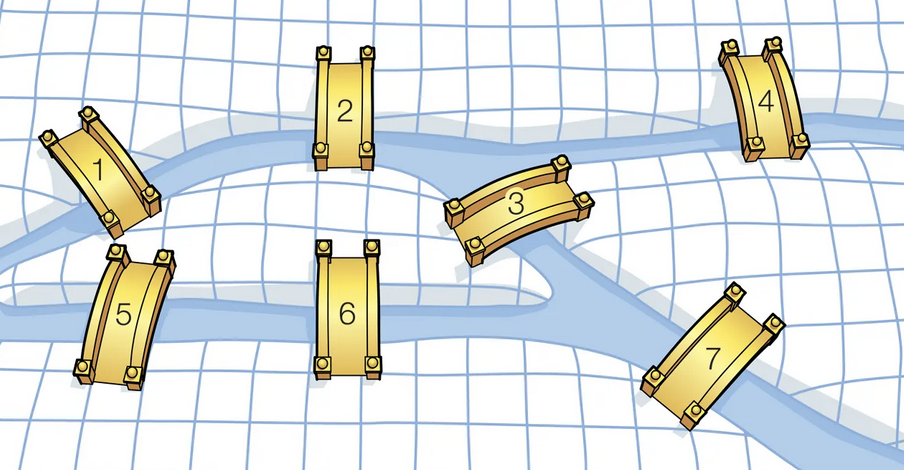
\includegraphics[scale=0.4]{img/bridges.png}
        \caption{Bridges of Konigsberg} 
        \label{fig:bridges}
      \end{figure}
      It can be decomposed into this undirected graph. 
      \begin{figure}[H]
        \centering 
        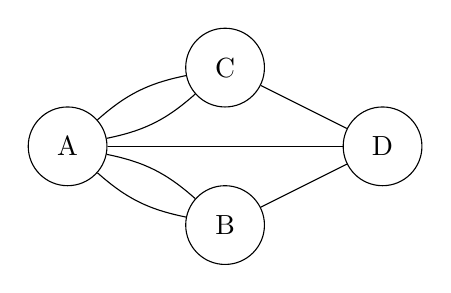
\begin{tikzpicture} 
          \tikzstyle{every node}=[circle, draw, minimum size=1cm]
          
          \node (A) at (0,0) {A};
          \node (B) at (2,-1) {B};
          \node (C) at (2,1) {C};
          \node (D) at (4,0) {D}; 
                
          \draw (A) to[bend left=15] (B);
          \draw (A) to[bend right=15] (B);
          \draw (A) to[bend left=15] (C);
          \draw (A) to[bend right=15] (C);
          \draw (A) -- (D);
          \draw (B) -- (D);
          \draw (C) -- (D);
        \end{tikzpicture}
        \caption{Graph representation. } 
        \label{fig:bridge_graph}
      \end{figure}
      Euler's observation is that except for start and end points, a talk leaves any vertex by different edge that the incoming edge. Therefore, the degree (number of edges incident on it) must have an even number, so all but 2 vertices must have an even degree. Since every vertex has an odd degree, there is no way of doing it. 
    \end{example}

    In addition to the \textit{adjacency list} representation, another way in which we represent a directed graph is through \textit{adjacency matrices}. 

    \begin{definition}[Adjacency Matrix]
      In a finite directed graph $(V, E)$, we can construct a bijection from $V$ to the natural numbers and so we label each element in $V$ with $i \in \mathbb{N}$. Then, we can construct a matrix $A$ such that 
      \begin{equation}
        A_{ij} = \begin{cases} 1 & \text{ if } (i, j) \in E \\ 0 & \text{ if } (i, j) \not\in E \end{cases}
      \end{equation}
    \end{definition}

    While the adjacency matrix does have its advantages and has a cleaner form, usually in sparse graphs this is memory inefficient due to there being an overwhelming number of $0$s. 

    \begin{definition}[Trees]
      An undirected graph $G(V, E)$ is a \textbf{tree} if 
      \begin{enumerate}
        \item $G$ is connected. 
        \item $G$ has no cycles.\footnote{This makes sense, since to get back to a previous vertex you must backtrack.}
      \end{enumerate}
      Removing the first requirement gives us the definition of a \textbf{forest}, which is a collection of trees. Conversely, if $G(V, E)$ is connected  and $|E| = n - 1$, then $G$ is a tree. 
    \end{definition}

    \begin{theorem}[Properties of Trees]
      If $G(V, E)$ is a tree, then 
      \begin{enumerate}
        \item There exists a $v \in V$ s.t. $d_v = 1$, called a \textbf{leaf node}. 
        \item $|E| = |V| - 1 = n - 1$. 
      \end{enumerate}
    \end{theorem}
    \begin{proof}
      The outlines are quite intuitive. 
      \begin{enumerate}
        \item There must be some leaf node since if there wasn't, then we would have a cycle. We can use proof by contradiction. 
        \item We can use proof by induction. We start off with one vertex and to construct a tree, we must add one edge and one vertex at every step, keeping this invariant.  
      \end{enumerate}
    \end{proof}

  \subsection{Exploration}

    Given two $v, s \in V$ either directed or undirected, how can we find the shortest path from $v$ to $s$? We can do with either with DFS or BFS. 

    \begin{definition}[DFS]
      The recursive algorithm is 
      \begin{lstlisting}
        visited = set() 
        def dfs(start): 
          if start not in visited: 
            visited.add(start) 
            # do something 
            neighbors = ... 
            for neighbor in neighbors: 
              dfs(neighbor)
      \end{lstlisting}

      The iterative algorithm uses a stack, which mirrors the function call stack. 
      \begin{lstlisting}
        visited = set() 

        def dfs(start): 
          toExplore = [] 
          current = start; 
          toExplore.append(current) 
          visited.add(current) 
          while toExplore: 
            current = toExplore.pop() 
            # Do something
            neighbors = ... 
            for neighbor in neighbors: 
              if neighbor not in visited: 
                visited.add(neighbor) 
                toExplore.append(neighbor)
      \end{lstlisting}
    \end{definition}

    \begin{theorem}[Runtime of DFS]
      The runtime of DFS is $O(n+m)$. 
    \end{theorem}
    \begin{proof}
      
    \end{proof}

    \begin{definition}[BFS]
      The iterative version is shown.\footnote{The recursive version of BFS is very nontrivial.}
      \begin{lstlisting}
        visited = set() 
        def bfs(start): 
          toExplore = collections.deque() 
          current = start; 
          toExplore.append(current) 
          visited.add(current) 
          while toExplore: 
            current = toExplore.popleft() 
            # Do something 
            neighbors = ... 
            for neighbor in neighbors: 
              if neighbor not in visited: 
                visited.add(neighbor) 
                toExplore.append(neighbor)
      \end{lstlisting}
    \end{definition}

    \begin{theorem}[Runtime of BFS]
      The runtime of BFS is $O(n+m)$. 
    \end{theorem}
    \begin{proof}
      To get the running time, we know that each vertex is popped only once from the queue, giving us $O(n)$. For each pop, we are exploring all the neighbors of $V$. 
      \begin{align}
        O \bigg( \sum_{v \in V} | \text{neighbors of } v| + 1\bigg) & = O \bigg( \sum_{v \in V} d_v + 1 \bigg) \\
                                             & = O (2 |E| + |V|) = O(m + n )
      \end{align}
      which is linear in input size!  
    \end{proof}

    The more straightforward application is in reachability. 

    \begin{example}[Reachability]
      Given a directed graph and a node $v$, find all nodes that are reachable from $v$. 
    \end{example}

    \begin{exercise}
      Prove that in any connected undirected graph $G = (V, E)$ there is a vertex $v \in V$ s.t. $G$ remains connected after removing $v$. 
    \end{exercise}
    \begin{proof}
      You can make a BFS tree from this graph, and there has to be a last layer. Just remove the node from this layer. 
    \end{proof}

    \begin{exercise}
      Give an example of a strongly connected directed graph $G = (V, E)$ s.t. that every $v \in V$, removing $v$ from $G$ gives a directed graph that is not strongly connected. 
    \end{exercise}
    
    \begin{exercise}[DPV 3.16]
    \end{exercise}
    \begin{proof}
      Do BFS but now recursively store the maximum of all the prerequisite courses plus 1 for the current course. 
    \end{proof}

  \subsection{Directed Acyclic Graphs and Topological Sorting}

    \begin{definition}[Directed Acyclic Graph]
      A DAG is a directed graph that has no cycles. Note that a DAG must have a node that has no in-edges. 
    \end{definition}

    To determine if a graph is a DAG, then we can brute force it by taking a node $s \in V$, running DFS/BFS, and if a neighbor is already in visited, return False. Then go through this for all starting nodes $s \in V$. This again has quadratic runtime. Can we do better? This introduces us to topological sorting. 

    It may be helpful to take a graph $G(V, E)$ and induce some partial order on the set of nodes $V$ based off of $E$. It turns out that we can do this for a specific type of graph. 
    
    \begin{definition}[Topological Sort]
      Given a directed acyclic graph (DAG), a linear ordering of vertices such that for every directed edge $u-v$, vertex $u$ comes before $v$ in the ordering is called a \textbf{topological sort}. It satisfies the facts: 
      \begin{enumerate}
        \item The first vertex must have an in-degree of $0$. 
        \item A topological sort is not unique. 
      \end{enumerate}
    \end{definition}

    \begin{example}[Simple Topological Sort]
      The graph below 
      \begin{figure}[H]
        \centering 
        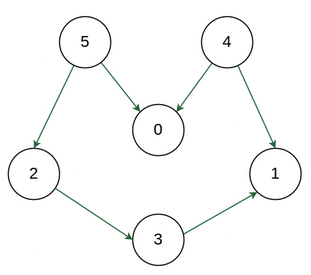
\includegraphics[scale=0.55]{img/top_sort.png}
        \caption{} 
        \label{fig:top_sort}
      \end{figure}
      can have the two (not exhaustive) topological sortings. 
      \begin{enumerate}
        \item $[5, 4, 2, 3, 1, 0]$
        \item $[4, 5, 2, 3, 1, 0]$
      \end{enumerate}
    \end{example}

    To determine if a graph is a DAG, note the following theorem. 

    \begin{theorem}[Topological Order and DAGs]
      $G$ has a topological order if and only if it is a DAG. 
    \end{theorem}
    \begin{proof}
      To prove that a DAG has a topological order, we use induction. Pick a $v$ such that its indegree is $0$. Then, delete $v$, and therefore $G \setminus v$ is also a DAG with a topological order since we are only deleting edges. We keep going. 
    \end{proof}

    Therefore, if we can successfully topologically sort, we know it is a DAG. So we can kill two birds with one stone. Let's see how this is implemented. We can do it iteratively and recursively (the proof above should hint that this can be recursive). 

    \begin{algo}[Iterative Topological Sort, Determine If Graph is DAG]
      The general idea is that we first find the node that as $0$ in-degree. From here, we can do DFS, and when we run out of neighbors to explore, then we push this into a queue. This is essentially a post-order traversal, where at the end are going to be the end nodes with no more neighbors, and the node we started from will be added last. Then we loop through and do this for all start nodes. We first need a slightly modified form of DFS. 

      \begin{algorithm}[H]
        \label{alg:iterative_top_sort}
        \begin{algorithmic}[1]
          \Require{Nodes $V$, adjacency list $E$}
          \State visited $\gets$ set()
          \State res $\gets$ stack() 
          \State is\_acyclic $\gets$ True

          \Function{DFS}{$v \in V$}
            \If{$v \neq $ visited}
              \State add $v$ to visited 
              \State $N_v \gets$ neighbors of $v$ 
              \For{$n \in N_v$}
                \If{$n \in $ visited} 
                  \State is\_acyclic $\gets$ False 
                \EndIf
                \State \Call{DFS}{$n$}
              \EndFor 
              \State push $v$ onto res
            \EndIf
          \EndFunction

          \State 

          \Function{TopologicalSort}{V, E}
            \For{$v \in V$} 
              \State DFS($v$)
            \EndFor
            \If{! is\_acyclic}
              \State \Return{False}
            \EndIf
            \State \Return{reversed of res}
          \EndFunction
        \end{algorithmic}
      \end{algorithm}
      Note that this runtime is $O(|V| + |E|)$ since we are just running DFS with a constant amount of work on top of each call. 
    \end{algo}

    \begin{algo}[Recursive Topological Sort]
      We want to see that while $G$ is nonempty, we want to find the $v \in V$ such that it has indegree $0$. Then place $v$ next in order, and then delete $v$ and all edges out of $v$. The problem is finding which vertex has indegree $0$ (if we brute force it by looking through all remaining nodes and edges, you have quadratic runtime). To do this fast, the idea is 
      \begin{enumerate}
        \item initially scan over all edges to store the indegrees of every node to a list \texttt{indeg}. 
        \item store all nodes with indegree $0$ to a queue. 
        \item Run through the queue, and during each loop, when we remove a node, we look at all of its out-nodes $s$ and decrement \texttt{indeg[s]}. If \texttt{indeg[s] = 0}, then add it to the queue. 
      \end{enumerate}
      \begin{algorithm}[H]
        \label{alg:recursive_top_sort}
        \begin{algorithmic}[1]
          \Require{Nodes $V$, Edges $E$}
          \State $q \gets$ queue() 
          \State indeg $\gets$ list() 
          \State visited $\gets$ 0
          \Function{Recur}{x}
            \State initialize the indeg and $q$ 

            \While{q is nonempty} 
              \State $v \gets$ pop(q) 
              \State visited += 1 
              \For{each $w \in E[v]$} 
                \State indeg[w] -= 1 
                \If{indeg[w] = 0} 
                  \State push w into q 
                \EndIf
              \EndFor
            \EndWhile

            \If{visited != |V|} 
              \State \Return{False}
            \EndIf

            \State \Return{True}
          \EndFunction
        \end{algorithmic}
      \end{algorithm}
      Notice that the inner for loop is $O(d(v) + 1)$, while we run over all $n$. So really, we are doing $O(n(d(v) + 1)) = O(m + n)$, where the plus $n$ comes from the constant work we are doing for each node. Note that if we have a non-DAG, then at some point the queue will be empty but we haven't processed all the vertices, at which point we can declare failure. 
    \end{algo}

    To end this, we can make a general statement about all directed graphs. 

    \begin{theorem}
      Every directed graph is a DAG of strongly connected components (SCC). 
    \end{theorem}

    This gives us a way to represent a directed graph with a collection of DAGs.\footnote{In fact, this Kosaraju's algorithm, can be done in linear time, though it is highly nontrivial.} An extension of topological sort is making a \textit{BFS tree}, which partitions a graph into layers that represent the number of steps required to go from a source vertex to a node. 

    \begin{algo}[BFS Tree]
      To construct a BFS tree, we just need to slightly modify the original BFS code.
      \begin{algorithm}[H]
        \label{alg:bfs_tree}
        \begin{algorithmic}[1]
          \Require{Nodes $V$, adjacency list $E$}
          \State visited = set() 
          \State layers = $\{v : 0 \mid v \in V \}$
          \Function{BFS}{start}
            \State layer $\gets 0$ 
            \State toExplore $\gets$ queue() 
            \State add (start, layer) to toExplore 
            \State add start to visited
            \While{toExplore} 
              \State curr, layer = pop from toExplore 
              \State layers[curr] = layer 
              \For{$n \in$ neighbors of curr} 
                \If{$n \not\in$ visited} 
                  \State add $n$ to visited 
                  \State add $(n, layer+1)$ to visited 
                \EndIf
              \EndFor
            \EndWhile 
          \EndFunction
        \end{algorithmic}
      \end{algorithm}
      This is simply BFS with constant extra work so it is $O(n + m)$. 
    \end{algo}

    So, a BFS tree is really just another way to topologically sort. Note the following properties. 
    \begin{enumerate}
      \item In a directed graph, no nodes can jump from layer $i$ to layers $j > i+1$, since if it could, then it would be in layer $i+1$. However, nodes can jump from layer $j$ back to any layer $i < j$, even skipping layers. 
      \item In a directed graph, going forward is the same as going back, so nodes can jump at most one layer forwards or backwards. 
    \end{enumerate}

  \subsection{Bipartite Graphs}

    Now we shall see a further application of BFS trees. 

    \begin{definition}[Bipartite Graph]
      A \textbf{bipartite graph} is an undirected graph $G(V, L)$ where we can partition $V = L \sqcup R$ such that for all $e = \{u, v\} \in E$, we have $u \in L, v \in R$.  
    \end{definition}

    We would like to devise some method to determine if an arbitrary graph is bipartite. 

    \begin{theorem}
      $G$ is bipartite if and only if all cycles in $G$ are even length. 
    \end{theorem}
    \begin{proof}
      Proving $(\implies)$ is quite easy since if we suppose $G$ has an odd length cycle, then we start packing vertices of a cycle into $L, R$, but by the time we came back to the start, we are forced to pack it into the wrong partition! 

      The converse is quite hard to prove, and we'll take it at face value. 
    \end{proof}

    Now in practice, how would we determine if all cycles are even length? This is where BFS shines. 

    \begin{algo}[Determine Bipartite On All Cycles of Even Length]
      The general idea is we first run BFS on the graph starting at $s \in V$, which divides it up into layers $L_1, \ldots, L_l$ representing the shortest path from $s$. Then for each layer $L_i \subset V$, we check if there are connections between two vertices $x, y \in L_i$. If there are connections, then this is not bipartite. If there are none, then this is bipartite since we can then color it. 

      \begin{algorithm}[H]
        \label{alg:determine_bipartite}
        \begin{algorithmic}[1]
          \Require{Nodes $V$, adjacency list $E$}
          \State visited = set() 
          \State layers = $\{v : 0 \mid v \in V \}$
          \Function{BFS}{start}
            \State layer $\gets 0$ 
            \State toExplore $\gets$ queue() 
            \State add (start, layer) to toExplore 
            \State add start to visited
            \While{toExplore} 
              \State curr, layer = pop from toExplore 
              \State layers[curr] = layer 
              \For{$n \in$ neighbors of curr} 
                \If{$n \not\in$ visited} 
                  \State add $n$ to visited 
                  \State add $(n, layer+1)$ to visited 
                \EndIf
              \EndFor
            \EndWhile 
          \EndFunction

          \State 

          \Function{Bipartite}{V, E}
            \State BFS(v) for some $v \in V$ 
            \For{$(u, v) \in E$} 
              \If{layers[u] == layers[v]} 
                \State \Return{False} 
              \EndIf 
            \EndFor 
            \State \Return{True}
          \EndFunction
        \end{algorithmic}
      \end{algorithm}
      Therefore, we run BFS, which is $O(n+m)$, and then to compare the edges, it is $O(m)$. 
    \end{algo}

    Bipartiteness is actually a special case of \textit{coloring problems}. Given a graph with $k$ colors, can I color it so that every neighbor has a different color than the original node? It may seem like at first glance that we can do the same method and look at the layers again, but it turns out that 3-coloring is hard. More specifically it is an NP-complete problem, which colloquially means that there isn't much of a better way than a brute-force solution. However, it turns out that according to the \textit{4 color theorem}, any map can be colored with 4 colors. 

  \subsection{Strongly Connected Graphs}

    Now how do we find out if a directed graph is strongly connected? The straightforward solution would be to take each vertex $v \in V$, run BFS to find the set of vertices reachable from $v$, and do this for every vertex. The total running time is $O(n(n+m))$, which is quadratic. Note that for an undirected graph this is trivial since we just run DFS/BFS once. 

    \begin{theorem}
      $G$ is strongly connected if and only if for any $v \in V$, 
      \begin{enumerate}
        \item all of $V$ is reachable from $v$. 
        \item $v$ is reachable from any $s \in V$
      \end{enumerate}
    \end{theorem}

    \begin{algo}[Determine if Graph is Strongly Connected]
      Using the theorem above, we can run BFS/DFS twice: one on the original graph and one on the reversed graph, consisting of all edges directed in the opposite direction. 
      \begin{algorithm}[H]
        \label{alg:strongly_connected}
        \begin{algorithmic}[1]
          \Require{Nodes $V$, Adjacency list $E$}
          \Function{StronglyConnected}{$s \in V$}
            \State visited $\gets$ set() 
            \State BFS(s) 
            \If{visited != $V$} 
              \State \Return{False}
            \EndIf
            \State visited $\gets$ set() 
            \State reverse all edges in $E$ 
            \State BFS(s) 
            \If{visited != $V$} 
              \State \Return{False}
            \EndIf
            \State \Return{True}
          \EndFunction
        \end{algorithmic}
      \end{algorithm}
      The running time is just running BFS twice plus the time to reverse the edges, so it is $O(n+m)$. 
    \end{algo}

  \subsection{Shortest Path}

    In the shortest path, you are given a \textit{weighted} (positive integer) directed graph and your goal is to find a path from $s$ to $t$ with the smallest length. This is where we use Dijkstra's. What we can do to brute force is just replace a edge with length $k$ to $k$ edges of length $1$, and we run BFS on this. However, this is not efficient. This is where we introduce Dijkstra. The following is how it is introduced in class. 

    \begin{algo}[Primitive Dijkstra]
      We can keep a temporarily list $\pi$ of the shortest path we have found so far, and a permanent list \texttt{dist} keeping track of all paths we know are for sure the shortest path. 
      \begin{algorithm}[H]
        \label{alg:dik_in_class}
        \begin{algorithmic}[1]
          \Require{Graph $G(E, V)$}
          \State $S \gets \{s\}$  \Comment{set of nodes that we know for sure is shortest}
          \State dist[s] = 0 and the rest very large numbers \Comment{our final list}
          \State $\pi[v] = w_{sv}$ for all $v \in V$ \Comment{initialize list with neighboring nodes from start $s$}
          \Function{Dijkstra}{s}
            \State $u = \mathrm{argmin}_{v \notin S} \pi[v]$ \Comment{Find node having minimum accum weight so far}
            \State add $u$ to $S$ \Comment{This node must be shortest so add to $S$}
            \State $\mathrm{dist}[u] = \pi[u]$ \Comment{Now we can update its shortest path in dist}
            
            \For{$v \not\in S$} \Comment{Look at all neighbors of $u$ and update those not in}
              \State $\pi[v] \gets \min\{\pi[v], d[u] + w_{wv}\}$ \Comment{$S$ since those in $S$ are all guaranteed to be shortest}
            \EndFor
          \EndFunction
        \end{algorithmic}
      \end{algorithm}
    \end{algo}

    The problem is line 5 above. We don't want this linear search time since it makes the whole thing quadratic, so rather than a list, we can implement a heap, resulting in the code below. 

    \begin{algo}[Dijkstra's Algorithm]
      The general idea is to run a graph traversal like BFS but when you reach a new vertex $v$, you can store the accumulated time it took to get to $v$ and store for all neighbors the accumulated time it will take to get to each of those neighbors. If it is less than what we have currently, then we have found a shorter path and we should update this. 
      \begin{algorithm}[H]
        \label{alg:dijkstra}
        \begin{algorithmic}[1]
          \Require{Nodes $V$, Edges $E$}
          \Function{Dijkstra}{s}
            \State dist $\gets$ list of size $|V|$ with $+\infty$ \Comment{Initialize a list of large numbers}
            \State dist[$s$] $\gets$ 0 \Comment{The starting node has dist $0$}
            \State predecessors $\gets$ $\{v : None \mid v \in V \}$
            \State toExplore $\gets$ minheap() \Comment{A priority queue of (weight, node)}
            \State add $(0, s)$ to toExplore

            \While{toExplore} 
              \State (curr\_dist, curr\_node) $\gets$ pop from toExplore 
              \If{curr\_dist > dist[curr\_node]} 
                \State continue 
              \EndIf 

              \For{neighbor, weight $\in E[curr]$} 
                \State new\_dist $\gets$ curr\_dist + weight
                \If{new\_dist < dist[neighbor]} 
                  \State dist[neighbor] = new\_dist
                  \State predecessors[neighbor] = curr\_node
                  \State push (new\_dist, neighbor) onto toExplore
                \EndIf
              \EndFor
            \EndWhile
            \State \Return{distances, predecessors}
          \EndFunction
        \end{algorithmic}
      \end{algorithm}

      You essentially push $n$ times and pop $m$ times, and the time per push and pop is $\log_2 (n)$. Therefore, the total time to push is $n \log(n)$ and to pop is $m \log (n)$, making the total runtime $O(log(n) (n+m))$. 

    \end{algo}

    The first example gotten in class ignores the distances and just attempts to modify the distances in the heap itself (through the decrease key operation). This takes $2 \log_2 (n)$, but if we use a heap with $d$ children, we can modify the runtime to $d \log_d (n)$. Therefore, the total runtime with tunable parameter $d$ is 
    \begin{equation}
      O\big( (m + nd) \log_d (n)\big)
    \end{equation}
    which can be minimized if we set $d = m/n$, so $O(m \log_{m/n} n)$, where for dense graphs $m/n$ is large and so it can behave roughly in linear time $\Theta(m)$. 

  \subsection{Negative Weighted Graphs} 

    Now let's extend this problem to find the shortest path in negative weighted graphs. Before we think of a solution, we must make sure that there is no cycle that has a negative accumulated path. Otherwise, this problem becomes ill-defined, so we first assume that such a shortest path exists. 

    At first glance, we may just think of adding $\min(v)$, the minimum value to every node so that this now just becomes a regular positive graph and run BFS on it. However, this does not work since we are not adding a constant number over all paths (it is proportional to the number of nodes in the path). 

    Another way we can think of is just run Dijkstra. However, if it is looking at two paths. We can have $s \xrightarrow{2} b$ and $s \xrightarrow{5} a \xrightarrow{-4} b$. Dijkstra will immediately go to $b$ thinking that it is the shortest path, since that's how far it see. So we need to look far into the future. Therefore, after an arbitrarily long path length, you could get a negative length that just kills your accumulator.  

    Another way we can do is to use dynamic programming. 

    \begin{theorem}[Bellman Equations]
      We write the \textbf{Bellman equations}. 
      \begin{align}
        d[v] & = \min_{w} \{ d[w] + l_{w v}\}
      \end{align}
      with $d[s] = 0$ for the starting vertex. The solution has a unique solution that finds the shortest path from $s$ to any $v \in V$.    
    \end{theorem}
    \begin{proof}
      Note that $d[w] + l_{wv}$ is the length from some path from $s \mapsto v$ that goes through $w$. The minimum of it must be the shortest path over all $w \in V$. Suppose the shortest path goes through fixed $x$. If there exists a shorter path from $s \mapsto x$, then replace $d[x]$ by this shortest path. Therefore, 
      \begin{equation}
        d[v] = d[x] + l_{xv} \leq d[w] + l_{wv} \implies d[v] = \min_{w} \{d[w] + l_{w v}\}
      \end{equation}
      To prove uniqueness, suppose there are some other solutions $\pi$ where $\pi[v] \neq d[v]$ for some $v$. But this cannot be the case by definition since $d[v] <= \pi[v]$ for all $v$. 
    \end{proof}

    \begin{theorem}
      Given the shortest paths, we can lay out this graph like a tree where $l_{ab} = l_{a a_1} + l_{a_1 a_2} + \ldots + l_{a_l b}$. 
    \end{theorem}

    So how do we actually implement this? 

    \begin{algo}[Shortest Path in Possibly Negative Weighted Graph]
      
      \begin{algorithm}[H]
        \label{alg:neg_weighted_short_path}
        \begin{algorithmic}[1]
          \Require{Nodes $V$, Edges $E$}
          \Function{ShortPath}{V, E}
            \State res $\gets$ list(0) of large numbers of size $|V|$. 
            \State res[$s$] = 0
            \State predecessors $\gets \{v : None | v \in V\}$

            \While{$\exists (u, v)$ s.t. res[v] > res[u] + $l_{u v}$ } 
              \State res[$v$] $\gets$ res[u] + $l_{uv}$
              \State predecessor[v] $\gets$ u
            \EndWhile

          \EndFunction
        \end{algorithmic}
      \end{algorithm}
      This is guaranteed to converge and stop after a finite number of steps since at every iteration, a path will either 
      \begin{enumerate}
        \item get updated from infinity to a path length 
        \item get reduced from a path length to a shorter path length
      \end{enumerate} 
      And we will have to reach the shortest path length at which point we can't reduce it further.\footnote{This algorithm is also called \textit{policy iteration} in reinforcement learning and is analogous to gradient descent.} 

      Computing the runtime is a bit tricky, since we can look at the same edge twice since minimum paths may have been updated in the middle. Therefore this list \texttt{res} may reduce very slowly. For example, let the length of each edge $|l_e| \leq L$. Then in the worst case, res[s] can be initialized to $(n-1) L$ representing the max path across all nodes, and we can decrease by $1$ in each step. So over all nodes, we can decrease so that each res[s] becomes $-(n-1)L$, meaning that we are doing on the order of $2 n^2 L$ iterations. This is too slow, especially for non-distributed settings. 

    \end{algo}

    A better way is to not be so random about how we choose the $(u, v)$ in the while loop. Notice how we can lay out the shortest paths like a tree, so we can work in layers. The next algorithm implements this. 

    \begin{algo}[Bellman-Ford Algorithm]
      We think of going in rounds indexed by $t$, and at every round, we are iterating through all the nodes and updating the shortest path of $v$ using the shortest path of $w$ included in all in-neighbors of $v$. At most, we will need to update this at most $n$ times, which will guarantee convergence.  
      \begin{algorithm}[H]
        \label{alg:bellman_ford}
        \begin{algorithmic}[1]
          \Require{Nodes $V$, Edges $E$}
          \State $\pi \gets$ list(0) of large numbers of size $|V|$. 
          \State $\pi[s] = 0$

          \Function{BellmanFord}{x}
            \For{$t = 1, \ldots, n-1$}
              \For{$v \in V$} 
                \State $\pi^{(t)} [v] \gets \min_w \{ \pi^{(k-1)} [v], \pi^{(k-1)}[w] + l_{wv}\}$
              \EndFor 
            \EndFor
          \EndFunction
        \end{algorithmic}
      \end{algorithm}
      The runtime is easier to see. 
      \begin{enumerate}
        \item The step in the inner loop looks over the set of nodes of size $\mathrm{indeg}(v)$. 
        \item Looping over all the nodes in the inner for loop means that we are going over all edges, so $O(m)$. 
        \item The outer for loop goes through $n-1$ times, so the total runtime is $O(nm)$. 
      \end{enumerate}
    \end{algo}

    At first glance, this problem seems like it isn't too different from Dijkstra, but there is a 50-year conjecture that this cannot be improved to linear time. 
   
  \subsection{Spanning Trees} 

    \begin{definition}[Spanning Tree]
      Given an undirected graph $G(V, E)$, a \textbf{spanning tree} is a subgraph $T(V, E^\prime \subset E)$ that is 
      \begin{enumerate}
        \item a tree, and 
        \item spans the graph, i.e. is connected 
      \end{enumerate}

      \begin{figure}[H]
        \centering 
        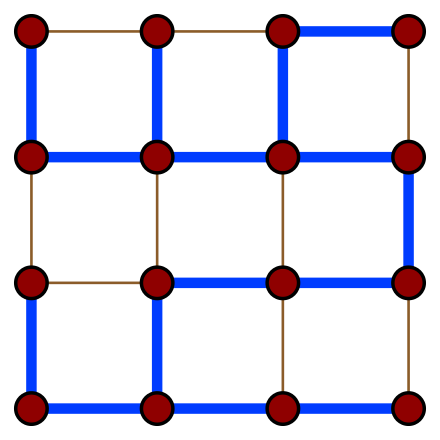
\includegraphics[scale=0.3]{img/spanning_tree.png}
        \caption{A spanning tree on a $4 \times 4$ grid graph. } 
        \label{fig:spanning_tree}
      \end{figure}
    \end{definition}

    Note that an unconnected graph will never have a spanning tree, but what about a connected graph? 

    \begin{theorem}[Spanning Trees of Connected Graphs]
      A connected graph will always have at least one spanning tree, not necessarily unique. 
    \end{theorem}

    Given a connected undirected weighted graph, we may want to find the \textbf{minimum spanning tree (MST)}, i.e. the spanning tree with edges $E^\prime$ such that the sum of the weights of all $e \in E^\prime$ is minimized.\footnote{An application of this is when we generally want to make sparse graphs. In a datacenter, wires can be expensive, so how I can minimize the length of wires to buy to construct a spanning subgraph?} How do we do this? 

    Let's try to apply what we already know: Dijkstra. If we run Dijkstra on the graph starting at $s \in V$, we can get the shortest path from $s$ to every other node in the graph. This will give us a tree, but it may not be minimum. 

    \begin{figure}[H]
      \centering 
      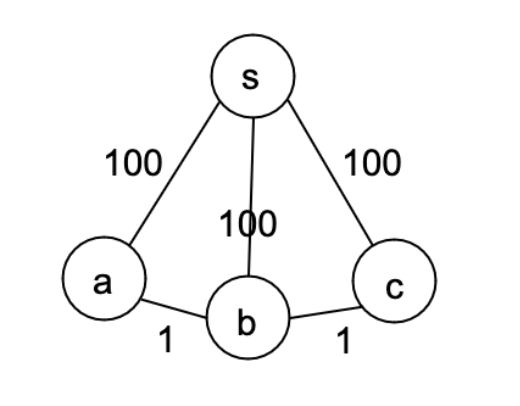
\includegraphics[scale=0.6]{img/dik_mst_prob.png}
      \caption{If we run Dijkstra on $s$, then our output will be a tree of cost $300$, even when the actual MST can be of cost $102$ starting from $a$.} 
      \label{fig:dik_mst_prob}
    \end{figure}

    It may seem like this is just a problem of where we start, but even this is not the case. 

    \begin{figure}[H]
      \centering 
      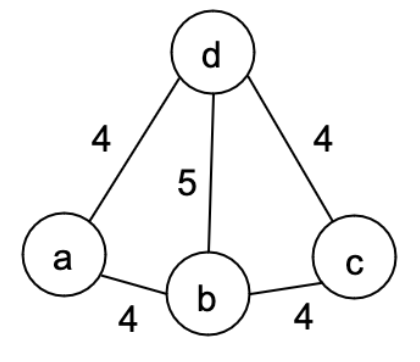
\includegraphics[scale=0.6]{img/dik_mst_prob2.png}
      \caption{No matter where we start from, we will never output the MST. The MST has cost $12$. If  we start from $b$ or $d$, we will get a tree of cost $13$. If we start from $a$ or $c$, we will get a tree of cost $16$.}
      \label{fig:dik_mst_prob2}
    \end{figure}

    \begin{definition}[Cuts]      
      Given graph $G(V, E)$, a \textbf{cut} is a partitioning of $V$ into $(S, V \setminus S)$. Furthermore, let $\mathrm{Cut}(S)$ be the number of edges with exactly one endpoint in $S$ and the other in $V \setminus S$. 
    \end{definition}

    \begin{theorem}[Cycles and Cuts]
      Given cycle $C \subset E$ in a graph and a cut $S \subset V$, 
      \begin{equation}
        | C \cap \mathrm{Cut}(S) | 
      \end{equation}
      is even. We can intuit this by visualizing the cycle as a long piece of looped string and a cut is a circle. The intersection between this circle and the string must be even since every time the cycle crosses through the cut, it must return back across the cut to the initial point.  
    \end{theorem}

    Now time for a bizarre theorem. 

    \begin{theorem}[Cut Property of MSTs]
      For all cuts $S \subset V$ of an undirected graph, the minimum cost edge in $\mathrm{Cut}(S)$ belongs to the MST. Furthermore, the converse is true: if we take all cuts and find all their minimum cost edges, these edges is precisely the MST! Therefore, an edge $e \in \mathrm{MST}$ iff $e$ is a min-cost edge for some cut. 
      \begin{figure}[H]
        \centering 
        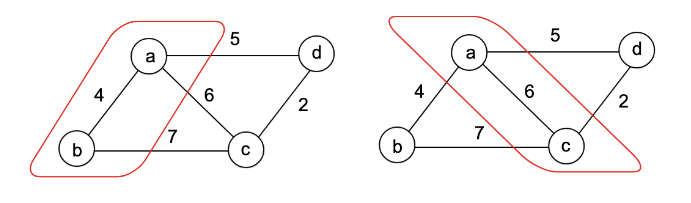
\includegraphics[scale=0.4]{img/mst_cut_prop.png}
        \caption{In the left cut, the edges are $(a,d), (b, c), (a, c)$. The minimum weight is $5$ on the $(a, d)$ edge, so it must be in the MST. For the right cut, $(c, d)$ must be in the MST. } 
        \label{fig:mst_cut_prop}
      \end{figure}
      The final part is that if we have all edge costs different, then we will have a \textit{unique} MST. 
    \end{theorem}
    \begin{proof}
      We use a greedy approach and prove by contradiction. Suppose that this is not true, i.e. there exists a cut $S$ with minimum cost edge $e$, and $e \not\in \mathrm{MST}$. Then, there exists some other edge $e^\prime \in \mathrm{Cut}(S)$ that is in the MST, since the MST is spanning and it must cross over to connect the whole graph. Well if we just put $e$ in and take $e^\prime$ out, we will still have a spanning tree since it connects the left spanning tree to the right spanning tree, and we now have a cheaper tree. So the original cannot be the MST in the first place. 

      To prove the converse, consider some edge $e$ in the MST and we must prove that it is the minimum cost edge in some cut. Note that if we take $e$ out, then it divides the MST into two connected components, and we can just define the cut as these subsets of nodes. So this is in $\mathrm{Cut}(S)$ for some $S \subset V$. We can also prove that this is minimal since if it wasn't the minimum cost edge for some cut, we could have taken it out and inserted a cheaper edge $e^\prime$ to begin with, getting a cheaper spanning tree.   
    \end{proof}

    \begin{algo}[Primitive Prim's Algorithm]
      We can just brute force this logic into an algorithm, which is not efficient. 
      \begin{algorithm}[H]
        \label{alg:primitive_prim}
        \begin{algorithmic}
          \Require{Graph $G(V, E)$}
          \State $r \gets \{\}$ 
          \Function{Solve}{x} 
            \For{all $S \subset V$} 
              \State add min-cost edge in $\mathrm{Cut}(S)$ to $r$
            \EndFor
            \State \Return{$r$}
          \EndFunction
        \end{algorithmic}
      \end{algorithm}
    \end{algo}

    It is clear that a cut is defined by a subset of $S$, so really the number of cuts a graph can have is $2^{|S| - 1}$, which is exponential in $n$. However, the minimum spanning tree isn't exponential since it must have $n-1$ edges, so there must be many cuts with the same minimum edge. 

    One way is to start with one vertex $a$ that contains the minimum cost edge $(a, b)$ across all edges.  This edge must be minimal and must be in the MST. Then we can look at the cut $S = \{a, b\}$ and look at that cut. We keep doing this, keeping track of the set of edges we need to look at after adding a new node to our cut. So the number of cuts I consider is equal to the number of edges in the spanning tree.

    \begin{figure}[H]
      \centering 
      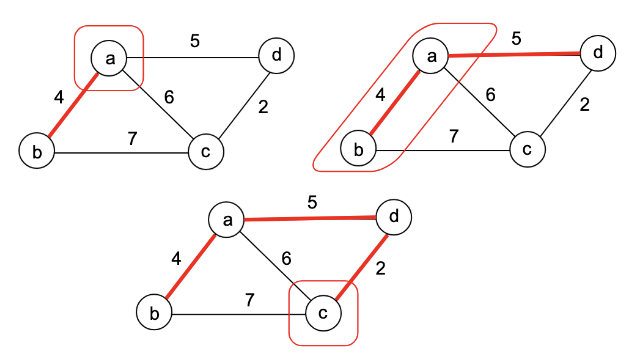
\includegraphics[scale=0.45]{img/prim.png}
      \caption{Step by step process of the method we mention above.} 
      \label{fig:prim}
    \end{figure}

    \begin{algo}[Prim's Algorithm to Find MST]
      It turns out that we can modify Dijkstra to solve it. 
      \begin{algorithm}[H]
        \label{alg:prim}
        \begin{algorithmic}[1]
          \Require{Graph $G(E, V)$}

          \Function{Prim}{s}
            \State $S \gets \{s\}$  \Comment{Our initial cut}
            \State $\pi[v] \gets$ list of size $|V|$ of $+\infty$ \Comment{$\pi[u]$ is min cost of getting from $u$ into the $S$}
            \State $\pi[v] = w_{sv}$ for all $v \in V$ \Comment{initialize list with neighboring nodes from start $s$}

            \While{$S \neq V$}
              \State $u = \mathrm{argmin}_{v \notin S} \pi[v]$ \Comment{Find node having minimum cost to reach from $S$}
              \State $S \gets S \cup \{u\}$ \Comment{Adding this node to $S$ to expand our cut}
              \For{$u \not\in S$} \Comment{Since we expanded $S$, our min reach distances}
                \State $\pi[u] \gets \min\{\pi[u], w_{wu}\}$ \Comment{must be updated. It can only get shorter} 
              \EndFor \Comment{through a path from new $u$, so compare them}
            \EndWhile
            
          \EndFunction
        \end{algorithmic}
      \end{algorithm}

      However, this is not efficient, so we can introduce a minheap to get the argmin step faster. 
      \begin{algorithm}[H]
        \caption{Not completely finished, need to update}
        \label{alg:prim_final}
        \begin{algorithmic}[1]
          \Require{Graph $G(E, V)$}

          \Function{Prim}{s}
            \State $S \gets \{s\}$  \Comment{Our initial cut}
            \State $T \gets \mathrm{heap}(\{(u, v, w) \in E \mid u = s\})$ \Comment{Our heap of edges connected to $S$}
            \State $\pi[v] \gets$ list of size $|V|$ of $+\infty$ \Comment{$\pi[u]$ is min cost of getting from $u$ into the $S$}
            \State $\pi[v] = w_{sv}$ for all $v \in V$ \Comment{initialize list with neighboring nodes from start $s$}

            \While{$S \neq V$}
              \State $u = \mathrm{argmin}_{v \notin S} \pi[v]$ \Comment{Find node having minimum cost to reach from $S$}
              \State $S \gets S \cup \{u\}$ \Comment{Adding this node to $S$ to expand our cut}
              \State update $T$
              \For{$v \in$ neighbors of $u$} \Comment{Since we expanded $S$, our min reach distances}
                \State $\pi[v] \gets \min\{\pi[v], w_{uv}\}$ \Comment{must be updated. It can only get shorter} 
              \EndFor \Comment{through a path from new $u$, so compare them}
            \EndWhile
            
          \EndFunction
        \end{algorithmic}
        Note that we run through all the nodes in line 6, and in line 10, we run through the neighbors of each edge, making this $O(n+m)$. However, to compute the argmin in line 7, it is a $O(\log{n})$ operation, so the total runtime is $O(m + n \log{n})$ operation. In class, it says running time is $\Theta(m \log_{m/n} {n})$. 
      \end{algorithm}
    \end{algo}

    If we were to try and construct this algorithm from scratch, we may take a greedy approach by incrementally adding the minimum cost edge from your cut. However, there is one thing to check: have we entered a cycle? Checking whether the next added node $a$ completes a cycle in $S \cup \{a\}$ is nontrivial. 

    \begin{theorem}[Cycle Property]
      For all cycles $C$, the max cost edge of $C$ does not belong to MST. 
    \end{theorem}

    Therefore, you can take $S$ and either add to it using the cut property or delete candidates from it using the cycle property. What is the best order to do this in? 

    \begin{algo}[Kruskal's Algorithm]
      This algorithm is faster and can be run faster than $O(m \log{n})$ time. The general idea is that we sort $e \in E$ in increasing cost, and for each $e \in E$, we use either the cut or cycle property to decide whether $e$ goes in or out. 
      \begin{algorithm}[H]
        \label{alg:kruskal}
        \begin{algorithmic}
          \Require{Graph $G(V, E)$}
          \Function{Kruskal}{V, E}
            \State sort $E$ in increasing cost 
            \State $T \gets \{\}$
            \For{$e \in E$}
              \If{$T \cup \{e\}$ does not have cycle} 
                \State $T \gets T \cup \{e\}$ \Comment{Cut property}
              \Else \Comment{Cycle property} 
                \State continue \Comment{discard $e$ since from sorting, this edge is heaviest in cycle}
              \EndIf
            \EndFor
          \EndFunction
        \end{algorithmic}
      \end{algorithm}
      The way to prove that this is correct is to show that every step you do is correct either because of one of the two properties. Say that so far, we have some edges in $V$ which forms a partition of $V = \sqcup_i T_i$ of disjoint trees (can be trees, one edge, or just single nodes). We are looking at the next biggest edge $e = (a, b)$. There are two possibilities. 

      \begin{enumerate}
        \item If $a, b$ are both in a single $T_i$, then this forms a cycle and can be thrown away since this is the max cost edge in the cycle by the cycle property. 
        \item If $a, b$ connect $T_i$ and $T_j$ for $i \neq j$, then this edge is in $\mathrm{Cut}(T_i)$ and is the minimum cost edge since the rest of the edges in $\mathrm{Cut}(T_i)$ come next in the sorted $E$. Therefore this must be included by the cut property. 
      \end{enumerate}
    \end{algo}

    \begin{algo}[Traveling Salesman Problem (TSP)]

      It's not like finding a tree, but we want to find a path that visits everything. 
      
      \begin{algorithm}[H]
        \caption{}
        \label{alg:tsp}
        \begin{algorithmic}[1]
          \Require{}
          \State 
          \Function{tsp}{x}
          \EndFunction
        \end{algorithmic}
      \end{algorithm}
    \end{algo}

    Here is a way to cluster data, a surprising way to apply MSTs. It is the most widely used application, esp in data science. 

    \begin{algo}[Clustering Data]
      
      \begin{algorithm}[H]
        \caption{}
        \label{alg:clustering}
        \begin{algorithmic}[1]
          \Require{}
          \State 
          \Function{Func}{x}
          \EndFunction
        \end{algorithmic}
      \end{algorithm}
    \end{algo}

\section{Approximation Algorithms}

  \subsection{Greedy Algorithms}

\section{Linear Programming}

\end{document}
